\documentclass[a4paper,11pt]{article}
\usepackage[left=2.5cm, right=2.5cm, top=1.5cm, bottom=1.5cm]{geometry}
\usepackage{graphicx}
\usepackage{amssymb}
\usepackage{amsmath}
\usepackage[procnames]{listings}
\usepackage{xcolor}
\usepackage{hyperref}

\hypersetup{ %color attributes of citation, link, etc.
    colorlinks=true,
    linkcolor=blue,
    filecolor=gray,
    urlcolor=blue,
    citecolor=blue,
}

\setlength{\parindent}{0pt}


\newcommand{\matlab}{\textsc{Matlab}} %very important and totally necessary addition
\newcommand{\parallelsum}{\mathbin{\!/\mkern-5mu/\!}}

\newcommand\Item[1][]{%
  \ifx\relax#1\relax  \item \else \item[#1] \fi
  \abovedisplayskip=0pt\abovedisplayshortskip=0pt~\vspace*{-\baselineskip}}

%'codify' text for snippets
\usepackage{xcolor}
\definecolor{codegray}{gray}{1}
\newcommand{\code}[1]{\colorbox{codegray}{\texttt{#1}}}

\definecolor{keywords}{RGB}{255,0,90}
\definecolor{comments}{RGB}{0,0,113}
\definecolor{p_red}{RGB}{160,0,0}
\definecolor{p_green}{RGB}{0,150,0} 
\lstset{language=Python, 
        basicstyle=\ttfamily\small, 
        keywordstyle=\color{keywords},
        commentstyle=\color{comments},
        stringstyle=\color{p_red},
        showstringspaces=false,
        identifierstyle=\color{p_green},
		procnamekeys={def,class}}

\graphicspath{ {./images/} }
           
\begin{document}
\title{\LARGE{\textbf{ENGR222 Assignment 1}}}
\author{Niels Clayton : 300437590}
\date{}
\maketitle
\hrule

\begin{enumerate}
    \item Consider the parametric equation: $$ (x,y) = (8sin(t), 2t-sin(2t)) $$ over the interval $ 0 \leq t \leq 2\pi $

    \begin{enumerate}
        \item Determine the location at $ t=0 , \frac{\pi}{4}, \frac{\pi}{2}, \frac{3\pi}{4}, \pi, \frac{5\pi}{4}, \frac{3\pi}{2}, \frac{7\pi}{4}, 2\pi$ and use this to draw a rough sketch of the curve.
        
        % Insert image
        \begin{center}
            \fbox{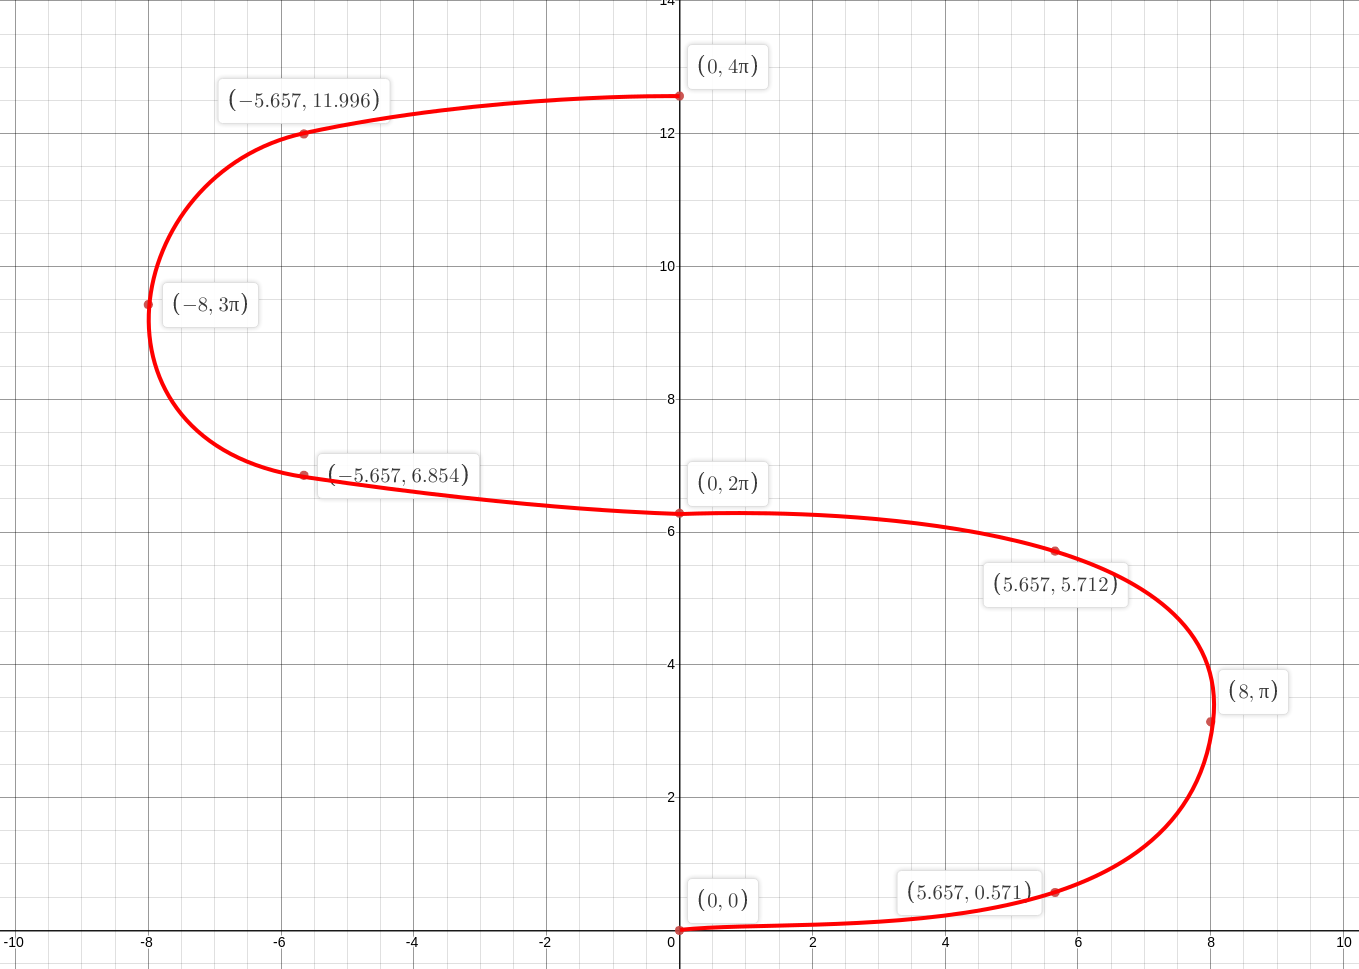
\includegraphics[width=0.8\textwidth]{image1.png}}
        \end{center}

        \item Find the unit tangent vector to the curve when $t = \frac{\pi}{6} $

        % Equation align
        \begin{align*}
            \left(f'(t), g'(t)\right) &= \left( 8 cos(t), 2 - 2 cos(2t)\right)\\
            t = \frac{\pi}{6} : \left(f'(t), g'(t)\right) &= (6.928203, 1)\\
        \end{align*}

        Calculate the unit tangent vector:
        \begin{align*}
            \frac{(f'(t), g'(t))}{||(f'(t), g'(t))||} &= \frac{(6.928203, 1)}{\sqrt{6.928203^2 + 1}} = \left( \frac{6.928203}{7}, \frac{1}{7}\right)\\
        \end{align*}

        \item Determine an equation describing the tangent line at $t = \frac{\pi}{6}$
        
        \begin{align*}
            &= \left( f(t), g(t) \right) + t \frac{(f'(t), g'(t))}{||(f'(t), g'(t))||}\\
            &= (4, 0.181) + t \cdot \left( \frac{6.928203}{7}, \frac{1}{7}\right)\\
            &= \left( \frac{6.928203 \cdot t}{7} + 4, \frac{t}{7} + 0.181 \right)
        \end{align*}

        \item Determine an equation describing the normal line at $t = \frac{\pi}{6}$

        \begin{align*}
            &= \left( f(t), g(t) \right) + t \frac{(-g'(t), f'(t))}{||(f'(t), g'(t))||}\\
            &= (4, 0.181) + t \cdot \left( \frac{-1}{7}, \frac{6.928203}{7}\right)\\
            &= \left( 4 - \frac{t}{7},  0.181 +\frac{6.928203 \cdot t}{7} \right)
        \end{align*}

        \item Calculate the arc length over the interval $0 \leq t \leq 2\pi$
        
        \begin{align*}
            L &= \int_{0}^{2\pi}\sqrt{f'\left(t\right)^{2}\ +\ g'\left(t\right)^{2}}\operatorname{dt}\\
            &= \int _0^{2\pi }\:\sqrt{\left(8cos\left(t\right)\right)^2+\left(2-2cos\left(2t\right)\right)^2} \operatorname{dt}\\
            &= \int_{0}^{2\pi}\sqrt{64\cos\left(t\right)^{2}+\left(2-2\cos\left(2t\right)\right)^{2}}\operatorname{dt}\\
            &= \int_{0}^{2\pi}\sqrt{\left(32\cos\left(2t\right)+32\right)+\left(4+4\cos\left(2t\right)^{2}-8\cos\left(2t\right)\right)}\operatorname{dt}\\
            &=\int_{0}^{2\pi}\sqrt{4\cos\left(2t\right)^{2}+24\cos\left(2t\right)+36}\operatorname{dt}\\
            &=\int_{0}^{2\pi}\sqrt{4\left(\cos\left(2t\right)^{2}+6\cos\left(2t\right)+9\right)}\operatorname{dt}\\
            &= \int_{0}^{2\pi}\sqrt{4\left(\cos\left(2t\right)+3\right)^{2}}\operatorname{dt}\\
            &= \ 2\int_{0}^{2\pi}\left(\cos\left(2t\right)+3\right)\operatorname{dt}\\
            &= \Big| sin(2t) + 6t \Big|^{2\pi}_{0}\\
            &= (0 + 12\pi) - (0 + 0)\\
            &= 12\pi \approx 37.6991\\
        \end{align*}

    \end{enumerate}

    \item Consider the curve described by the vector valued function
    $$ \bar{r}(t) = \frac{1}{4}(e^{2t}-2t)\bar{i} + e^t\bar{j} $$

    \begin{enumerate}
        \item   Find a point on the curve for which $\bar{r}(t) \cdot \bar{j}=2$
        \begin{align*}
            \bar{r}(t) \cdot \bar{j} &= e^t = 2\\
            t = \ln(2)&=0.693147\\
            \bar{r}(\ln(2)) &= (0.635, 2)
        \end{align*}
        \newpage

        \item Determine the unit tangent vector to the curve (for arbitrary t)
        
        \begin{align*}
            \bar{r}'(t) &= \frac{1}{4}(2e^{2t}-2)\bar{i} + e^t\bar{j}\\
            \bar{T}(t) &= \frac{\bar{r}'(t)}{|| \bar{r}'(t) ||}\\\\
            &= \frac{\frac{1}{4}(2e^{2t}-2)\bar{i} + e^t\bar{j}}{\sqrt{ (\frac{1}{4}(2e^{2t}-2))^2 + e^{2t}}}\\\\
            &= \frac{(e^{2t}-1)} {(e^{2t}+1)} \bar{i} + \frac{2e^t}{ (e^{2t}+1)} \bar{j}
        \end{align*}

        \item  Determine the principal unit normal vector to the curve (for arbitrary t)
        
        \begin{align*}
            \bar{N}(t) &= \frac{\bar{T}'(t)}{|| \bar{T}'(t) ||}\\\\
            \bar{T}'(t) &= \frac{ 2e^{2t}(e^{2t}+1) - 2e^{2t}(e^{2t}-1)}{ (e^{2t}+1)^2 } \bar{i} + 
            \frac{ 2e^t (e^{2t}+1) - 2e^t \cdot 2e^{2t}}{ (e^{2t}+1)^2 }\bar{j}\\\\
            \bar{T}'(t) &= \frac{4e^{2t}}{(e^{2t}+1)^{2}}\bar{i} + \frac{2e^{t}-2e^{3t}}{(e^{2t}+1)^{2}}\bar{j} \equiv \operatorname{sech}^2(t)\bar{i} + (-\operatorname{sech}(t) \operatorname{tanh}(t))\bar{j}\\\\
            || \bar{T}(t) || &= \sqrt{ \operatorname{sech}^4(t) + (-\operatorname{sech}(t) \operatorname{tanh}(t)) ^2 } = \sqrt{\operatorname{sech}^2(t)} \\\\
            \bar{N}(t) &= \frac{\operatorname{sech}\left(t\right)^{2}\overline{i}+\left(-\operatorname{sech}\left(t\right)\tanh\left(t\right)\right)\overline{j}}{\sqrt{\operatorname{sech}^2(t)}}
        \end{align*}

        \item  Determine the curvature of the curve (for arbitrary t)
        
        \begin{align*}
            \kappa(t) &= \frac{|| \bar{T}'(t) ||}{|| \bar{r}'(t) ||}\\\\
            &= \frac{2 \sqrt{\operatorname{sech}^2(t)}}{(e^{2t}+1)} \\
        \end{align*}

        \newpage

        \item  Determine the arc length of the curve over $ 0 \leq t \leq 3 $
        
        \begin{align*}
            L &= \int_{0}^{3} || \bar{r}'(t) ||\\
              &= 2 \int_{0}^{3} (e^{2t}+1) \operatorname{dt}\\
              &= \Big| \frac{1}{4}(e^{2t} + 2t) \Big|^3_0\\
              &= \frac{1}{4}((e^6 + 6) - (1+0))\\
              &= 102.107\\
        \end{align*}

    \end{enumerate}

    \item  Quick questions\\
    
    \begin{enumerate}
        \item Determine the arc length parametrisation of:
        $$ (f(t),g(t),h(t)) = (3t,t-2,-5t+7) $$
        with $t = 0$ as the starting/reference point

        \begin{align*}
            \left(f'(t), g'(t), h'(t)\right) &= \left( 3, 1, -5 \right)\\
            ||\left(f'(t), g'(t), h'(t)\right)|| &= \sqrt{3^2 + 1^2 + (-5)^2}=\sqrt{35}\\\\
            s &= \int^t_0 || \bar{r}'(u) || \operatorname{du} = \int^t_0 \sqrt{35} \operatorname{du}\\
            &= \Big| \sqrt{35}\operatorname{u} \Big|^t_0 = \sqrt{35}t\\\\
            t &= \frac{1}{\sqrt{35}}s\\
            (f(s),g(s),h(s)) &= \left( \frac{3}{\sqrt{35}}s, \frac{1}{\sqrt{35}}s -2, \frac{-5}{\sqrt{35}}s +7 \right)\\
        \end{align*}

        \newpage
        \item  Determine the arc length parametrisation of:\\
        $$ \bar{r}(t) = (5\cos(t) + 3)\bar{i} + (-5\sin(t) + 2)\bar{j} $$\\
        using $t = 0$ as the starting/reference point

        \begin{align*}
            \bar{r}'(t) &= (-5\sin(t))\bar{i} + (-5\cos(t))\bar{j}\\
            || \bar{r}'(t) || &= \sqrt{(-5\sin(t))^2 + (-5\cos(t))^2}\\
            &= \sqrt{25(\sin(t)^2 + \cos(t))^2}\\
            &= \sqrt{25}\sqrt{1} = 5\\\\
            s &= \int^t_0 || \bar{r}'(t) ||\operatorname{du} = \int^t_0 5 \operatorname{du}\\
            &= \Big| 5\operatorname{u} \Big|^t_0 = 5t\\\\
            t &= \frac{s}{5}\\
            \bar{r}(s) &= \left(5\cos\left(\frac{s}{5}\right) + 3\right)\bar{i} + \left(-5\sin\left(\frac{s}{5}\right) + 2\right) \bar{j}\\
        \end{align*}

        \item Find the unit tangent vector to:\\
        $$ \bar{r}(t) = (\sqrt{2}\cos(t))\bar{i} + (\sin(t))\bar{j} + (\sin(t))\bar{k} $$

        at $t = \frac{\pi}{3}$

        \begin{align*}
            \bar{T}(t) &= \frac{\bar{r}'(t)}{|| \bar{r}'(t) ||}\\\\
            \bar{r}'(t) &= (- \sqrt{2}\sin(t))\bar{i} + (\cos(t))\bar{j} + (\cos(t))\bar{k}\\
            || \bar{r}'(t) || &= \sqrt{(- \sqrt{2}\sin(t))^2 + (\cos(t))^2+ (\cos(t))^2}\\
            &= \sqrt{2 \sin^2(t) + 2 \cos^2(t)}\\
            &= \sqrt{2}\sqrt{1} = \sqrt{2}\\\\
            \bar{T}(t) &= \frac{(- \sqrt{2}\sin(t))\bar{i} + (\cos(t))\bar{j} + (\cos(t))\bar{k}}{\sqrt{2}}\\
            \bar{T}\left(\frac{\pi}{3}\right) &= \frac{(- \sqrt{2}\sin(\frac{\pi}{3}))\bar{i} + (\cos(\frac{\pi}{3}))\bar{j} + (\cos(\frac{\pi}{3}))\bar{k}}{\sqrt{2}}\\\\
            \bar{T}\left(\frac{\pi}{3}\right) &= \frac{\left( -\frac{\sqrt{6}}{2} \right) \bar{i} + \left(\frac{1}{2}\right) \bar{j} + \left(\frac{1}{2}\right)\bar{k} }{\sqrt{2}}
        \end{align*}

        \newpage
        \item An alternative formula for the binormal vector is:
        $$ \bar{B}(t) = \frac{\bar{r}'(t) \times \bar{r}''(t)}{|| \bar{r}'(t) \times \bar{r}''(t) ||} $$
        Use this to find the binormal vector to:
        $$ \bar{r}(t) = t\bar{i} -t^3\bar{j} + t^2\bar{k} $$
        At the point $t = 1$

        \begin{align*}
            \bar{r}'(t) &= \bar{i} - 3t^2\bar{j} + 2t\bar{k}\\
            \bar{r}''(t) &= 0\bar{i} - 6t\bar{j} + 2\bar{k}\\\\
            \bar{r}'(t) \times \bar{r}''(t) &=  
            \begin{vmatrix}
                \bar{i} & \bar{j} & \bar{k}\\
                1 & -3t^2 & 2t \\
                0 & -6t & 2
            \end{vmatrix}\\
            &= \begin{vmatrix}
                -3t^2 & 2t \\
                -6t & 2
            \end{vmatrix} \bar{i}
            -\begin{vmatrix}
                1 & 2t\\
                0 & 2
            \end{vmatrix} \bar{j}
            +  \begin{vmatrix}
                1 & -3t^2\\
                0 & -6t
            \end{vmatrix}\bar{k}\\
            &=6t^2\bar{i} - 2\bar{j} - 6t\bar{k} \\\\
            || \bar{r}'(t) \times \bar{r}''(t) || &= \sqrt{36t^4 + 4 + 36t^2}\\\\
            \bar{B}(t) &= \frac{6t^2\bar{i} - 2\bar{j} - 6t\bar{k}}{\sqrt{36t^4 + 4 + 36t^2}}\\\\
            \bar{B}(1) &= \frac{6\bar{i} - 2\bar{j} - 6\bar{k}}{\sqrt{76}}
        \end{align*}
        
        \newpage
        \item Find the minimum and maximum curvature for the curve described by:
        
        \begin{align*}
            \bar{r}(t) &= (3\sin(t) +2)\bar{i} + (2\cos(t)+1)\bar{j}\\
            \kappa(t) &= \frac{|| \bar{r}'(t) \times \bar{r}''(t) ||}{|| \bar{r}'(t) ||^3}\\\\
            \bar{r}'(t) &= 3\cos(t)\bar{i} -2\sin(t)\bar{j}\\
            \bar{r}''(t) &= -3\sin(t)\bar{i} -2\cos(t)\bar{j}\\\\
            \bar{r}'(t) \times \bar{r}''(t) &= 
            \begin{vmatrix}
                \bar{i} & \bar{j} \\
                3\cos(t) & -2\sin(t) \\
                -3\sin(t) & -2\cos(t) 
            \end{vmatrix}\bar{k}\\
            &= \left( -6\cos^2(t) - 6\sin^2(t) \right)\bar{k} = -6\bar{k}\\\\
            || \bar{r}'(t) \times \bar{r}''(t) || &= \sqrt{-6^2} = 6\\\\
            || \bar{r}'(t) || &= \sqrt{(3\cos(t))^2 + (-2\sin(t))^2}\\
            &= \sqrt{9\cos^2(t) + 4\sin^2(t)}\\
            &= \sqrt{5\cos^2(t) + 4} \\\\
            \kappa(t) &= \frac{6}{\left(\sqrt{5\cos^2(t) + 4}\right)^3}
        \end{align*}

        Since the curvature $\kappa$ is periodic on $\pi$ due to the $\cos^2(t)$, we know that the minimum and maximum will fall on $\frac{\pi}{2}$ and $\pi$. In the following plot we can see that $t=\frac{\pi}{2}$ is the maximum, and $t=\pi$ is the minimum.

        % Insert image
        \begin{center}
            \fbox{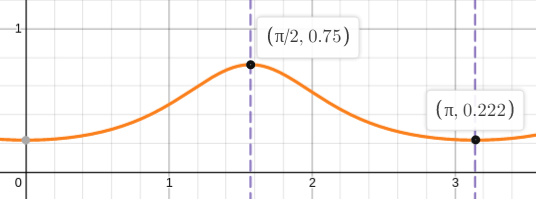
\includegraphics[width=0.8\textwidth]{image2.png}}
        \end{center}

        $$ \kappa(\frac{\pi}{2}) = \frac{6}{\left(\sqrt{5\cos^2(\frac{\pi}{2}) + 4}\right)^3}= 0.75$$
        $$ \kappa(\pi) = \frac{6}{\left(\sqrt{5\cos^2(\pi) + 4}\right)^3} = 0.22\bar{2}$$

    \end{enumerate}

    \newpage
    \item Suppose a roller coaster follows a path described by:
    $$ \bar{r}(t) = \frac{1}{5}t(20-t)\bar{i} + \frac{t^2}{50}(20-t)\bar{j} + \frac{t}{50}(10-t)(20-t)\bar{k} $$\\

    \begin{enumerate}
        \item Determine the velocity vector of the roller coaster (for arbitrary $t$)
        \begin{align*}
            \bar{r}'(t) &= (4 - \frac{2t}{5}) \bar{i} + \frac{t}{50}(40-3t)\bar{j} + \left(\left(\frac{3t^2}{50}-\frac{6t}{5}\right)+4\right)\bar{k}\\
        \end{align*}

        \item Determine the speed when $t = 5$
        \begin{align*}
            \bar{r}'(5) &= (4 - 2) \bar{i} + \frac{5}{50}(40-15)\bar{j} + \left(\left(\frac{75}{50}-\frac{30}{5}\right)+4\right)\bar{k}\\
            &= 2\bar{i} + 2.5\bar{j} - 0.5\bar{k}\\
            || \bar{r}'(5) || &= \sqrt{2^2 + 2.5^2 + -0.5^2} = 3.162278\\
        \end{align*}

        \item  Determine the acceleration vector of the roller coaster (for arbitrary $t$)

        \begin{align*}
            \bar{r}''(t) &= -\frac{2}{5}\bar{i} + (\frac{4}{5} - \frac{3t}{25})\bar{j} + \frac{3t-30}{25}\bar{k}\\
        \end{align*}

        \item Determine the curvature of curve followed by the roller coaster when $t = 5$
        
        \begin{align*}
            \kappa(t) &= \frac{|| \bar{r}'(t) \times \bar{r}''(t) ||}{|| \bar{r}'(t) ||^3}\\\\
            \bar{r}'(5) &= 2\bar{i} + 2.5\bar{j} - 0.5\bar{k}\\
            \bar{r}''(5) &= -0.4\bar{i} + 0.2\bar{j} - 0.6\bar{k}\\
            || \bar{r}'(5) ||^3 &= 31.622787\\\\
            \bar{r}'(5) \times \bar{r}''(5) &=  
            \begin{vmatrix}
                \bar{i} & \bar{j} & \bar{k}\\
                2 & 2.5 & -0.5 \\
                -0.4 & 0.2 & -0.6
            \end{vmatrix}\\
            &= \begin{vmatrix}
                2.5 & -0.5 \\
                0.2 & -0.6
            \end{vmatrix} \bar{i}
            -\begin{vmatrix}
                2 & -0.5\\
                -0.4 & -0.6
            \end{vmatrix} \bar{j}
            +  \begin{vmatrix}
                2 & 2.5\\
                -0.4 & 0.2
            \end{vmatrix}\bar{k}\\
            &= -1.4\bar{i} -1.4\bar{k} + 1.4\bar{k}\\\\
            || \bar{r}'(5) \times \bar{r}''(5) || &= \sqrt{-1.4^2 -1.4^2 + 1.4^2} = \frac{7\sqrt{3}}{5}\\\\
            \kappa(5) &= \frac{\frac{7\sqrt{3}}{5}}{31.622787} = 0.712696
        \end{align*}

    \end{enumerate}


\end{enumerate}
\end{document}